%change default fontsize to be smaller
\documentclass[8pt]{extarticle}
\usepackage{graphicx} % Required for inserting images
\usepackage{amsmath}
\usepackage{geometry} % Package for adjusting page margins
\usepackage{algorithm}
\usepackage{algpseudocode}
\usepackage{url}
\usepackage{hyperref}
\usepackage{booktabs}

% Adjust page margins
\geometry{
  margin=1in, % Set all margins to 1 inch (adjust as needed)
  top=0.7in   % Make top margin smaller
}


% \setlength{\floatsep}{6pt plus 2pt minus 2pt}      % Space between floats
% \setlength{\textfloatsep}{6pt plus 2pt minus 2pt}    % Space between floats and text
% \setlength{\intextsep}{6pt plus 2pt minus 2pt}       % Space above and below in-text floats

\setlength{\textfloatsep}{5pt plus 1pt minus 1pt}
\setlength{\floatsep}{5pt plus 1pt minus 1pt}
\setlength{\intextsep}{5pt plus 1pt minus 1pt}


% Reduce spacing around math environments
\setlength{\abovedisplayskip}{3pt}
\setlength{\belowdisplayskip}{3pt}
\setlength{\abovedisplayshortskip}{2pt}
\setlength{\belowdisplayshortskip}{2pt}


\title{Investigating the Discrete Fourier Transform and Fast Fourier Transform}
\author{Zihe Liu \\ zl559 \\ University of Cambridge}
\date{7 March 2025}

\begin{document}

\maketitle

\section{Outline}

We analyze the theoretical properties of both the \textit{Discrete Fourier Transform} (DFT) and the optimized \textit{Fast Fourier Transform} (FFT), and estimate their algorithmic complexity. Following Objective 6 in Experiment A4 Lab of Part 1B Integrated Coursework, we implement both the DFT and FFT in \texttt{MATLAB}, thereafter measuring their algorithmic complexity in the context of processing signal response to vibrations. We also investigate the effect of windowing functions on the accuracy of the frequency analysis using DFT.

\newpage
\section{Discrete Fourier Transform}

\subsection{Theory}
The DFT converts a finite-length time-domain signal into its frequency-domain representation. For an input signal $x[n]$ of length $N$, where $0 \le n \le N-1$, the DFT is defined as:

\begin{equation}
    X[k] = \sum_{n=0}^{N-1} x[n]\, W_N^{kn}, \quad 0 \le k \le N-1
\label{eq:DFT}
\end{equation}

where $W_N=e^{-j\frac{2\pi}{N}}$ is the $N$-th principal root of unity, and $X[k]$ is component at frequency $kf_s/N$ with sampling frequency $f_s$. We can rewrite $X[k]$ as an inner product:

\begin{equation*}
    X[k] = \left[ 1 \quad e^{-j\frac{2\pi k}{N}} \quad \ldots \quad e^{-j\frac{2\pi k}{N}(N-1)} \right] 
    \begin{bmatrix} 
    x[0] \\
    x[1] \\
    \vdots \\
    x[N-1]
    \end{bmatrix} 
    = \left[ 1 \quad W_N^k  \quad \ldots \quad W_N^{(N-1)k} \right] 
    \begin{bmatrix}
    x[0] \\
    x[1] \\
    \vdots \\
    x[N-1]
    \end{bmatrix}
\end{equation*}

By varying $k$ from $0$ to $N-1$, we can collate all outputs ${X[k]}$ into a vector $\mathbf{X}$, collate all inputs $x[n]$ into a vector $\mathbf{x}$, to get:

\begin{equation}
    \mathbf{X}=\mathbf{W}\mathbf{x}, \quad
\mathbf{W} = 
\begin{bmatrix}
1 & 1 & 1 & \cdots & 1 \\
1 & W_N & W_N^2 & \cdots & W_N^{N-1} \\
1 & W_N^2 & W_N^4 & \cdots & W_N^{2(N-1)} \\
\vdots & \vdots & \vdots & \ddots & \vdots \\
1 & W_N^{N-1} & W_N^{2(N-1)} & \cdots & W_N^{(N-1)(N-1)}
\end{bmatrix}
\end{equation}

where $\mathbf{W}$ is the DFT matrix.

\subsection{Complexity}

\begin{algorithm}
\caption{Matrix-Vector DFT Implementation}
\begin{algorithmic}[1]
\Function{DFT}{$\mathbf{x}$}
    \State $N \gets \text{length}(\mathbf{x})$
    \State $\mathbf{W} \gets \text{zeros}(N, N)$ \Comment{Initialize DFT matrix}
    
    \For{$k = 0$ \textbf{to} $N-1$}
        \For{$n = 0$ \textbf{to} $N-1$}
            \State $\mathbf{W}[k,n] \gets e^{-j2\pi kn/N}$
        \EndFor
    \EndFor
    
    \State $\mathbf{X} \gets \mathbf{W} \cdot \mathbf{x}$ \Comment{Matrix-vector multiplication}
    \State \Return $\mathbf{X}$
\EndFunction
\end{algorithmic}
\label{alg:dft}
\end{algorithm}

Direct computation of $\mathbf{X}$ requires $(N-1)^2$ complex multiplications and $N(N-1)$ complex additions, as in Algorithm \autoref{alg:dft}. Since multiplication is more compute-intensive than addition, the asymptotic complexity is dominated by multiplication, giving $O(N^2)$.

\section{Fast Fourier Transform}

\subsection{Theory}

The radix-2 FFT algorithms work by dividing the DFT into 2 DFTs of length $N/2$ each, and iterating. We introduce the simplest variant, called the \textit{Decimation-In-Time} (DIT) algorithm. DIT begins by splitting $x[n]$ into two parts --- one for the even-indexed values $x[2n]$ and one for the odd-indexed values $x[2n + 1]$. Define two $N/2$-point signals $x_{even}[n]$ and $x_{odd}[n]$ as
\begin{equation*}
x_{even}[n] = x[2n], \quad x_{odd}[n] = x[2n + 1], \quad 0 \leq n \leq N/2-1
\end{equation*}

using the DFT of these 2 splits gives us:

\begin{align}
X[k] &= X_{even}[k] + W_N^{k} \cdot X_{odd}[k] \quad \text{for } 0 \leq k \leq \frac{N}{2} - 1 \\
X[k + N/2] &= X_{even}[k] - W_N^{k} \cdot X_{odd}[k] \quad \text{for } 0 \leq k \leq \frac{N}{2} - 1
\label{eq:fft_final}
\end{align}

The first computation with $+W_N^k$ give us the first half of the full DFT vector $\mathbf{X}$, while the second computation with $-W_N^k$ give us the second half of $\mathbf{X}$. The proof is laid out in the Appendix.

\subsection{Complexity}

\begin{algorithm}
\caption{Radix-2 Decimation-In-Time FFT Implementation}\label{alg:fft}
\begin{algorithmic}[1]
\Function{FFT}{$\mathbf{x}$}
    \State $N \gets \text{length}(\mathbf{x})$
    
    \If{$N = 1$}
        \State \Return $\mathbf{x}$ \Comment{Base case: return the single value}
    \EndIf
    
    \State $\mathbf{x}_{even} \gets \mathbf{x}[0:2:N-1]$ \Comment{Extract even-indexed elements (half of $\mathbf{x}$)}
    \State $\mathbf{x}_{odd} \gets \mathbf{x}[1:2:N-1]$ \Comment{Extract odd-indexed elements (other half of $\mathbf{x}$)}
    
    \State $\mathbf{X}_{even} \gets \text{FFT}(\mathbf{x}_{even})$ \Comment{Recursive call on even elements}
    \State $\mathbf{X}_{odd} \gets \text{FFT}(\mathbf{x}_{odd})$ \Comment{Recursive call on odd elements}
    
    \State $\mathbf{X} \gets \text{zeros}(N)$ \Comment{Initialize output vector}
    
    \For{$k = 0$ \textbf{to} $N/2-1$}
        \State $W_N^k \gets e^{-j2\pi k/N}$ \Comment{Twiddle factor}
        \State $\mathbf{X}[k] \gets \mathbf{X}_{even}[k] + W_N^k \cdot \mathbf{X}_{odd}[k]$ \Comment{First half of $\mathbf{X}$ }
        \State $\mathbf{X}[k+N/2] \gets \mathbf{X}_{even}[k] - W_N^k \cdot \mathbf{X}_{odd}[k]$ \Comment{Second half of $\mathbf{X}$}
    \EndFor
    
    \State \Return $\mathbf{X}$
\EndFunction
\end{algorithmic}
\end{algorithm}

We can follow the above procedure to split an $N$-point DFT into two $\frac{N}{2}$-point DFT, giving us Algorithm \autoref{alg:fft}. Let $A_c(N)$ and $M_c(N)$ denote respectively the number of complex additions and multiplications for computing the DFT of an $N$-point complex sequence $x[n]$. Let $N$ be a power of 2, $N = 2^k$. Then, we have
\begin{equation*}
    A_c(N) = 2 A_c(N/2) + N \quad , \quad M_c(N) = 2 M_c(N/2) + \frac{N}{2} - 1
\end{equation*}

as $N$ complex additions (addition of even and odd terms) and $\frac{N}{2} - 1$ complex multiplications ($W_N^{k} \cdot X_{odd}[k]$)  are required to put the two $N/2$-point DFTs together. Note that a 2-point DFT is simply a sum and difference $X[0] = x[0] + x[1] , \quad X[1] = x[0] - x[1]$. Hence, the starting conditions are $A_c(2) = 2$ and $M_c(2) = 0$. Solving the recursive equation yields
\begin{equation*}
A_c(N) = N \log_2 N  \quad , \quad M_c(N) = \frac{N}{2} \log_2 N - N + 1
\end{equation*}

% A single complex multiplication can be performed with 4 real multiplications and 2 real additions. A single complex addition can be performed with 2 real additions. Therefore,
% \begin{align*}
% M_r(N) &= 4 \cdot M_c(N) \\
% A_r(N) &= 2 \cdot M_c(N) + 2 \cdot A_c(N)
% \end{align*}

% which gives
% \begin{align*}
% M_r(N) &= 2N \log_2 N - 4N + 4 \\
% A_r(N) &= 3N \log_2 N - 2N + 2
% \end{align*}

Our overall complexity is $O(N\log N)$.

\section{Experiments}

\subsection{Complexity}

\begin{figure}[h]
    \centering
    \includegraphics[width=0.4\textwidth]{figures/complex.jpg}
    \caption{Execution time versus signal length $N$ for various implementations of DFT and FFT}
    \label{fig:complexity}
\end{figure}

\begin{table}[h]
    \centering
    \begin{tabular}{lccccc}
        \toprule
        Algorithm   & O(N)    & O(N²)   & O(N³)   & O(log N) & O(N log N) \\
        \midrule
        my-DFT     & 0.9208  & 0.9999  & 0.9864  & 0.4167   & 0.9417  \\
        my-FFT     & 0.9830  & 0.9657  & 0.9161  & 0.5634   & 0.9894  \\
        MATLAB-FFT & 0.8491  & 0.7141  & 0.6526  & 0.8537   & 0.8287  \\
        \bottomrule
    \end{tabular}
    \caption{R\textsuperscript{2} values for different complexity models.}
    \label{tab:R2}
\end{table}

To verify the theoretical complexity, we measured the execution time for computing the DFT over a range of signal lengths. For each signal length $N$, $N$ samples were taken from a 5Hz sine wave, and the DFT/FFT computation time recorded. We compare our implementation of Algorithm \autoref{alg:dft} as \texttt{my-DFT}, our implementation of Algorithm \autoref{alg:fft} as \texttt{my-FFT}, and the \texttt{MATLAB} FFT implementation as \texttt{MATLAB-FFT}. \autoref{fig:complexity} shows the measured execution times on a log-log plot. The FFT results clearly exhibit an $O(N\log N)$ scaling, while the DFT scales as $O(N^2)$. These experimental results confirm the significant computational advantage of using the FFT for large-scale problems. We also note the much more efficient implementation of \texttt{MATLAB} FFT, which uses the \texttt{FFTW} \footnote{This package is highly optimized to each machine and is written in low level C} package. \autoref{tab:R2} show the how well different models fit to data. Both FFT implementations fit well to $O(N)$ and $O(N\log N)$ models.

\subsection{Numerical Error}

\begin{figure}[h]
    \centering
    \includegraphics[width=0.4\textwidth]{figures/recon.jpg}
    \caption{Reconstruction error versus signal length $N$ for various implementations of DFT and FFT}
    \label{fig:recon}
\end{figure}

We evaluate numerical accuracy of both algorithms in \autoref{fig:recon} by measuring reconstruction error of the reconstructed signal $
\text{RMSE} = \sqrt{\frac{1}{N}\sum_{i=1}^{N}|x_i - \hat{x}_i|^2}$ where $x_i$ is the original signal and $\hat{x}_i$ is the reconstructed signal (using the \texttt{MATLAB} Inverse DFT function) Despite all errors falling within the $10^{-12}$ range, indicating high overall accuracy, the custom DFT implementation exhibits exponentially growing error with increasing sequence length. In contrast, both FFT implementations maintain consistently minimal error across all tested sequence lengths. The superior numerical stability of FFT algorithms is possibly due to its lower operation count (lower algorithmic complexity). Floating-point rounding errors accumulate more significantly in DFT.

\subsection{Windowing}

Since we can only sample signals for a finite time period, the truncated signal contains discontinuities. Discontinuities in the time domain become "ripples" in the frequency domain, known as spectral leakage. A "window function" smooths these edges, reducing unwanted spectral leakage. We experiment with 3 different windowing functions on a sine wave of 5Hz input frequency, and do a DFT on the the input force transducer data (Channel 1):

\begin{figure}[h]
\centering
% First image in its own minipage
\begin{minipage}{0.5\textwidth}
  \centering
  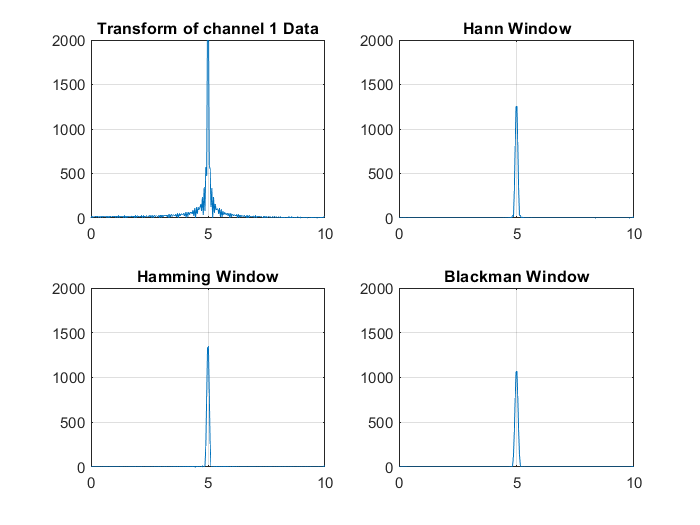
\includegraphics[width=0.7\linewidth]{figures/sin5_window.png}
\end{minipage}%
\hfill
% Second image in its own minipage
\begin{minipage}{0.5\textwidth}
  \centering
  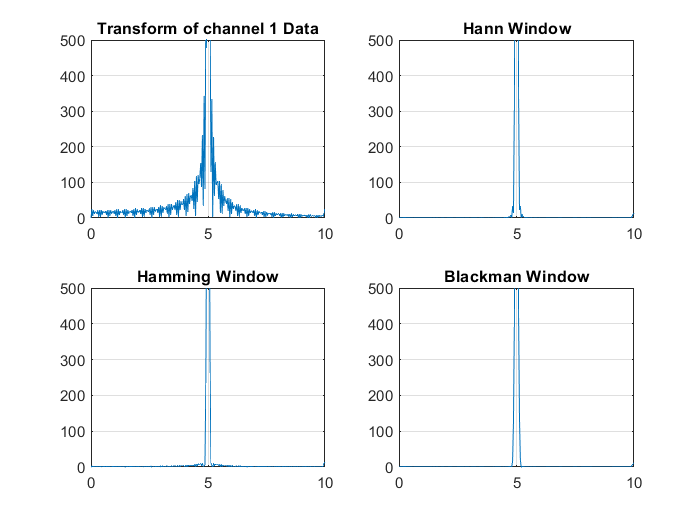
\includegraphics[width=0.7\linewidth]{figures/sin5_window_zoomed.png}
\end{minipage}
% A single caption for both images
\caption{Effect of windowing on amplitude and side lobe suppression.}
\label{fig:windowing}
\end{figure}

\begin{itemize}
    \item \textbf{Hann Window:} $0.5*(1-cos(2\pi n / (N - 1)))$
    \item \textbf{Hamming Window:} $0.54-0.46cos(2\pi n / (N - 1))$
    \item \textbf{Blackman-Harris Window:} $0.42-0.5cos(2\pi n / (N - 1))+0.8cos(4\pi n / (N - 1)))$
\end{itemize}

As seen in \autoref{fig:windowing}, the Han/Hamming window is effective and reducing unwanted frequences for smooth, continuous signals while the Blackman window is ideal for transient analysis with minimal leakage.



\section{Conclusion}

In this report, we investigated both theoretical and practical aspects of the DFT and the FFT. The analysis verified that the computational complexity of the direct DFT implementation scales as \(O(N^2)\), whereas our FFT implementation achieved the expected \(O(N \log N)\) complexity, offering a significant improvement in efficiency. Moreover, the FFT exhibited superior numerical stability. Selecting the appropriate windowing function is also crucial for accurate frequency analysis, with the Han or Hamming window recommended for most applications. All code available at \url{https://github.com/liuzihe02/dft-fft.git}.

\newpage
\appendix

\section*{Appendix: Derivation of FFT}
\label{app:fft_proof}

Consider again a $N$-point signal $x[n]$ of even length. The derivation of the DIT radix-2 FFT begins by splitting the $x[n]$ into two parts --- one part for the even-indexed values $x[2n]$ and one part for the odd-indexed values $x[2n + 1]$. Define two $N/2$-point signals $x_{even}[n]$ and $x_{odd}[n]$ as
\begin{equation*}
x_{even}[n] = x[2n], \quad x_{odd}[n] = x[2n + 1], \quad 0 \leq n \leq N/2-1
\end{equation*}

The DFT can be written as

\begin{align*}
X[k] &= \sum_{n=0 \atop n \text{ even}}^{N-1} x[n] W_N^{nk} + \sum_{n=0 \atop n \text{ odd}}^{N-1} x[n] W_N^{nk}\\
&= \sum_{n=0}^{N/2-1} x[2n] W_N^{2nk} + \sum_{n=0}^{N/2-1} x[2n + 1] W_N^{(2n+1)k}\\
&= \sum_{n=0}^{N/2-1} x_{even}[n] W_N^{2nk} + \sum_{n=0}^{N/2-1} x_{odd}[n] W_N^{(2n+1)k} \\
&= \sum_{n=0}^{N/2-1} x_{even}[n] W_N^{2nk} + W_N^{k} \cdot \sum_{n=0}^{N/2-1} x_{odd}[n] W_N^{2nk}\\
\end{align*}

Noting that $W_N^{2}=W_{N/2}$ or more generally $W_N^{2nk}=W_{N/2}^{nk}$,
\begin{align*}
X[k]&= \sum_{n=0}^{N/2-1} x_{even}[n] W_{N/2}^{nk} + W_N^{k} \cdot \sum_{n=0}^{N/2-1} x_{odd}[n] W_{N/2}^{nk}
\end{align*}

Recognizing that the $\frac{N}{2}$-point DFT of $x_{even}[n]$ and $x_{odd}[n]$ are given by:

\begin{equation*}
X_{even}[k] = \text{DFT}_{\frac{N}{2}}\{x_{even}[n]\} = \sum_{n=0}^{N/2-1} x_{even}[n] W_{N/2}^{nk} \quad , \quad X_{odd}[k] = \text{DFT}_{\frac{N}{2}}\{x_{odd}[n]\} = \sum_{n=0}^{N/2-1} x_{odd}[n] W_{N/2}^{nk}
\end{equation*}

we then obtain our core recursive equation:

\begin{equation}
    X[k] = X_{even}[k] + W_N^{k} \cdot X_{odd}[k]
    \label{eq:fft_int}
\end{equation}

Since $x_{even}[n]$ and $x_{odd}[n]$ are $N/2$-point signals with $ 0 \leq n \leq N/2-1$, their DFT are also only $N/2$-point signals. However, we require $0 \le k \le N-1$. We resolve this by noting their DFT coefficients are periodic with a period of $\frac{N}{2}$

\begin{equation*}
    X_{even}[k] = X_{even}\left[k + \frac{N}{2}\right], \quad X_{odd}[k] = X_{odd}\left[k + \frac{N}{2}\right]
\end{equation*}

This gives us

\begin{equation*}
    X[k] = 
    \begin{cases}
    X_{even}[k] + W_N^{k} \cdot X_{odd}[k], & \text{for } k = 0,1,\ldots,\frac{N}{2}-1 \\
    X_{even}\left[k-\frac{N}{2}\right] + W_N^{k} \cdot X_{odd}\left[k-\frac{N}{2}\right], & \text{for } k = \frac{N}{2},\frac{N}{2}+1,\ldots,N-1
\end{cases}
\end{equation*}

Noting $W_N^{k +\frac{N}{2}}=-W_{N}^{k}$, we write

\begin{equation*}
    X[k] = 
    \begin{cases}
    X_{even}[k] + W_N^{k} \cdot X_{odd}[k], & \text{for } k = 0,1,\ldots,\frac{N}{2}-1 \\
    X_{even}\left[k-\frac{N}{2}\right] - W_N^{k-\frac{N}{2}} \cdot X_{odd}\left[k-\frac{N}{2}\right], & \text{for } k = \frac{N}{2},\frac{N}{2}+1,\ldots,N-1
\end{cases}
\end{equation*}

finally giving us

\begin{align}
X[k] &= X_{even}[k] + W_N^{k} \cdot X_{odd}[k] \quad \text{for } 0 \leq k \leq \frac{N}{2} - 1 \\
X[k + N/2] &= X_{even}[k] - W_N^{k} \cdot X_{odd}[k] \quad \text{for } 0 \leq k \leq \frac{N}{2} - 1
\label{eq:fft_final}
\end{align}

The multipliers $W_N^k$ are known as \textit{twiddle factors}. The first computation with $+W_N^k$ give us the first half of the full DFT vector $\mathbf{X}$, while the second computation with $-W_N^k$ give us the second half of $\mathbf{X}$.


\newpage
\bibliographystyle{plain}  % or any style you prefer (e.g., alpha, abbrv)
\bibliography{references}
\nocite{*}

\end{document}
